\section{Supplementary Material}
\newcommand{\beginsupplement}{%
    \setcounter{table}{0}
    \renewcommand{\thetable}{S\arabic{table}}%
    \setcounter{figure}{0}
    \renewcommand{\thefigure}{S\arabic{figure}}%
}
\beginsupplement

\begin{figure}[!ht]
    \center
    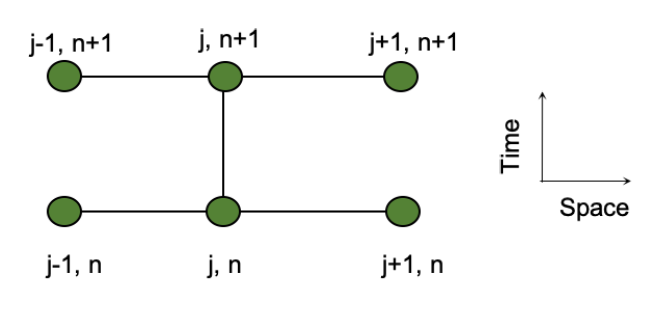
\includegraphics[width=0.3\textwidth]{figures/stencils}

    \caption{\textbf{Crank-Nicolson for a numerical solution}. A stencil is a geometric representation with nodes and edges, that represents the points of interest for the numerical approximation. The points of interest, which are the ones present in the equations, are shown in green. j and n are txhe current space and time points. The CN stencil as 1 spatial dimension and 1 temporal dimension, therefore its axes are time and space ($x$). }   \label{sup_fig1}
\end{figure}


\begin{figure}[!h]
    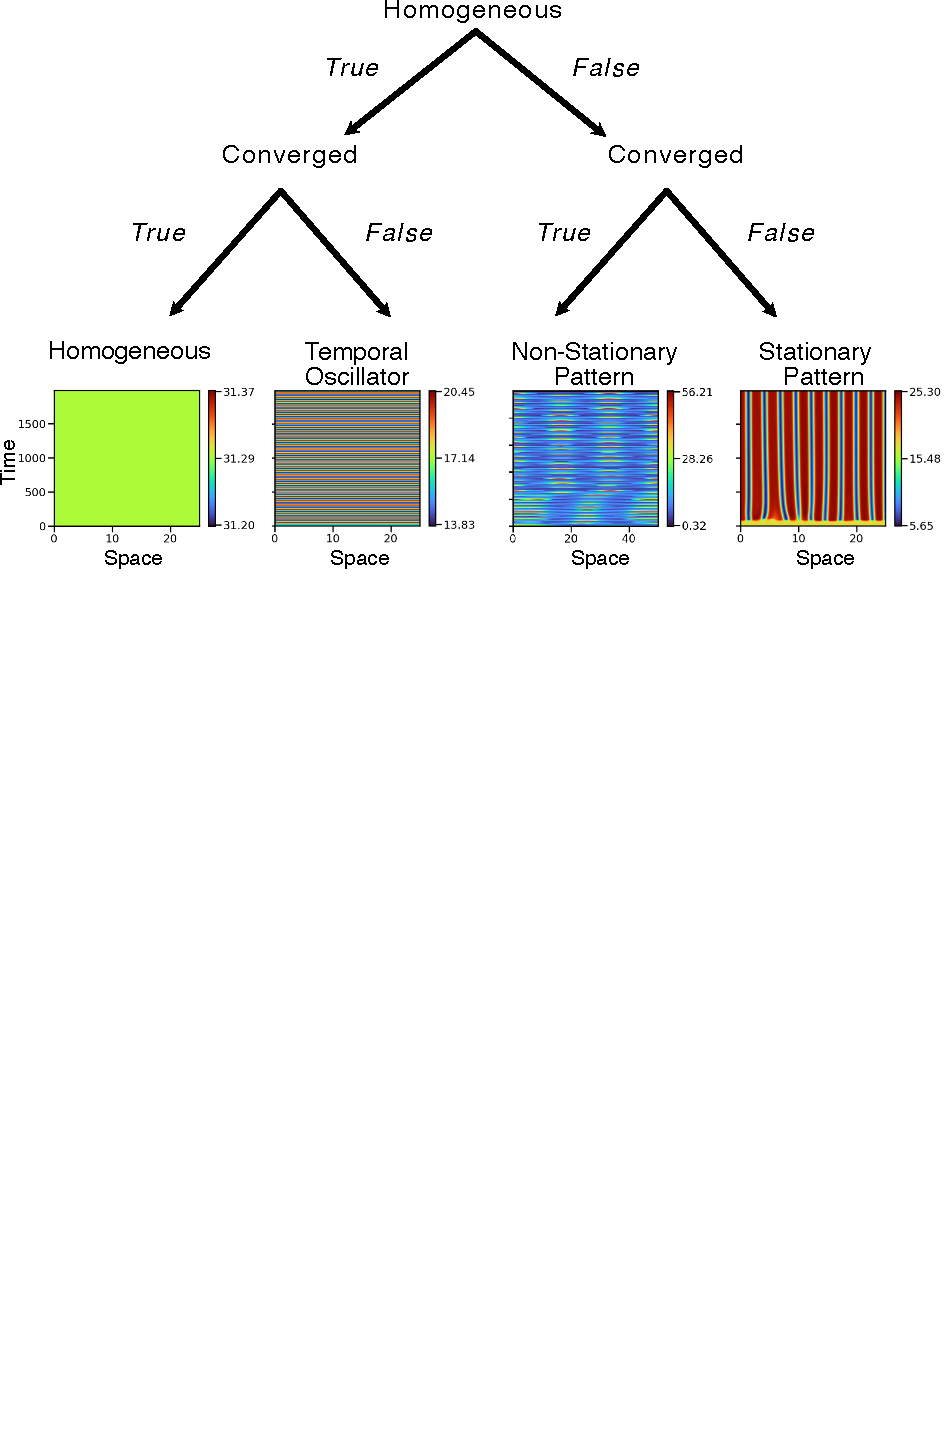
\includegraphics[width=1\textwidth]{figures/no_growth_classification}

    \caption{\textbf{Decision tree for pattern classification in non-growing domains with reflective boundaries}. A decision tree is based on two layers: spatial homogeneity and convergence. The numerical solutions for the four different pattern outcomes including a homogeneous, temporal oscillator, non-stationary pattern and stationary pattern are shown below.}
    \label{sup_fig2}
\end{figure}


\begin{figure}[!h]
    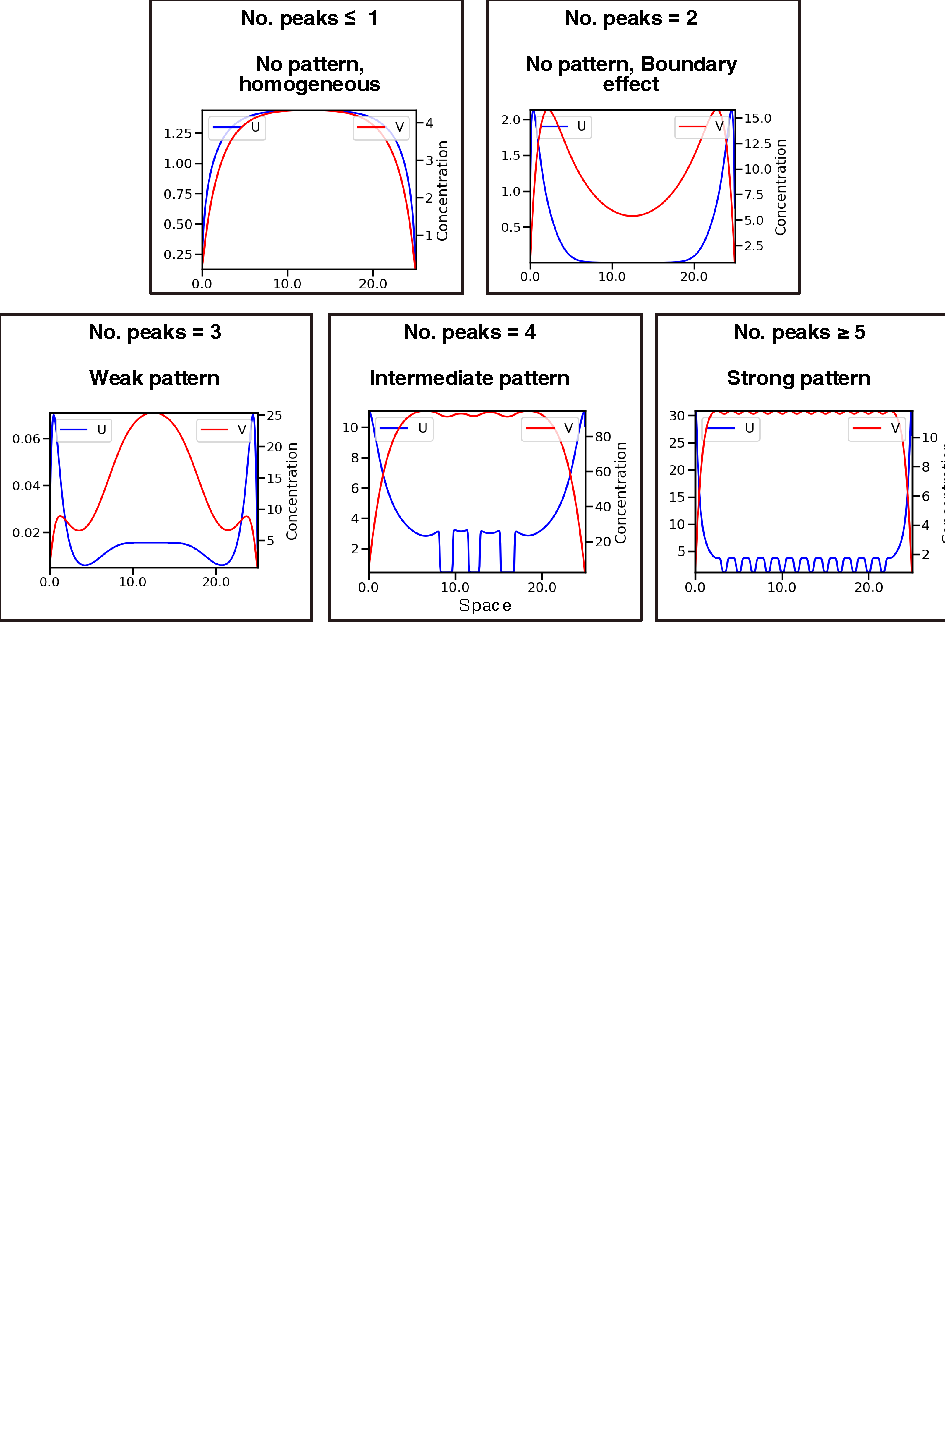
\includegraphics[width=1\textwidth]{figures/growth_classification}

    \caption{\textbf{Decision tree for pattern classification in non-growing domains with reflective boundaries}. A decision tree is based on two layers: spatial homogeneity and convergence. The numerical solutions for the four different pattern outcomes including a homogeneous, temporal oscillator, non-stationary pattern and stationary pattern are shown below.}
    \label{sup_fig3}
\end{figure}


\begin{figure}[!h]
    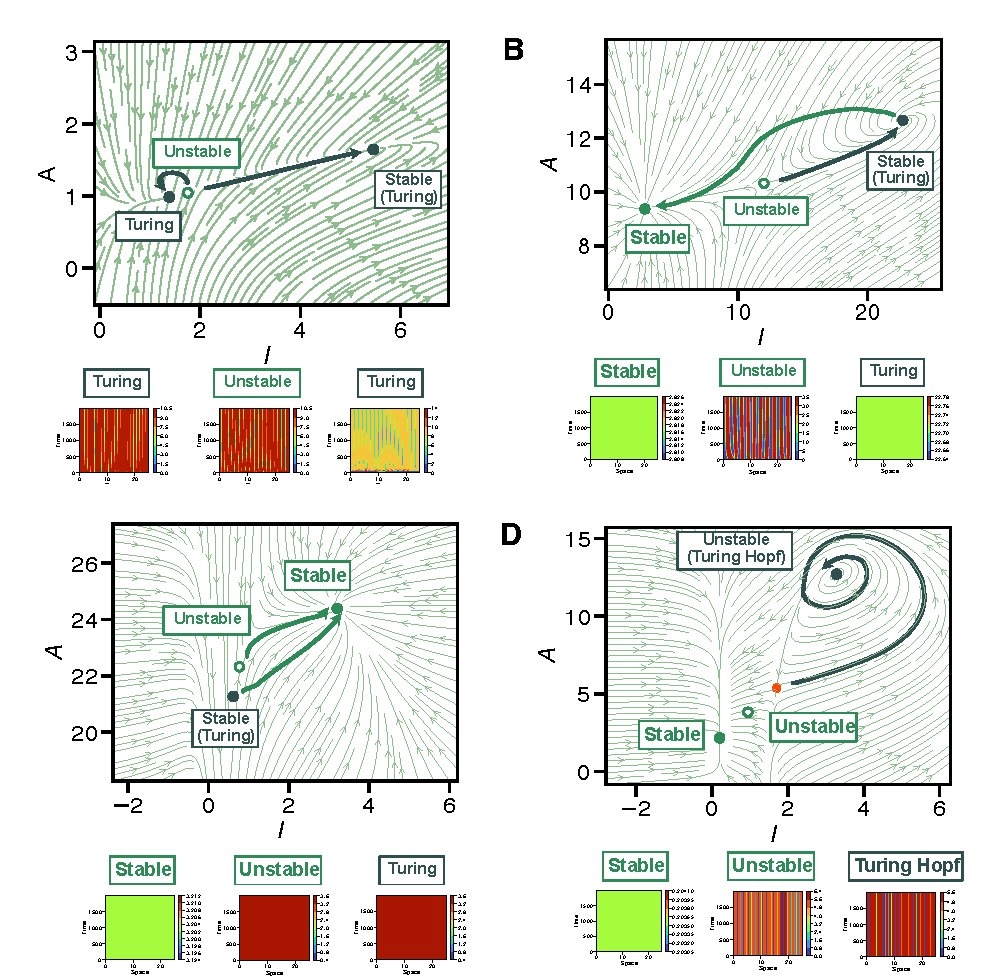
\includegraphics[width=1\textwidth]{figures/multistability_leftovers}

    \caption{\textbf{Other types of multistability dynamics.} \textbf{(A)} Unstable surrounded by Turing robustly converges into Turing. \textbf{(B)} Unstable produces pattern, while Turing loses pattern. \textbf{(C)} Multistability disrupts all patterns. \textbf{(D)} Turing I-Hopf attracts unstable and generates pattern}

    \label{sup_fig4}
\end{figure}

